%======================== USD Thesis Template ==============================%
% Made according to the guide, keeping in mind the guide was made for Word
% TODO: Make a copy of this file that can be used right away once everything is done
\documentclass[oneside,12pt]{book}


\usepackage{titlesec} % Manage chapter and sections
\usepackage{fontspec} % Manage fonts
\usepackage{fancyhdr} % Manage header styles
\usepackage{lipsum} % Lorem Ipsum
\usepackage{graphicx} % to add images
\usepackage[portrait, left=4cm, right=3cm, top=3cm, bottom=3cm]{geometry} % set margins
\usepackage{indentfirst} % indents first line after section
\usepackage{setspace}
\usepackage{listings} % Allow writing code
\usepackage{courier} % Code listing font family
\usepackage{import} % used to import files from different directories
\usepackage{float} % Adds more image float positions
\usepackage{pythontex} % Because
\usepackage[numbib]{tocbibind}
\usepackage[labelfont=bf, labelsep=period]{caption} % Manages captions. Changed to bold and separated using period
\usepackage{pdfpages} % Allows adding pdfs as pages
% \usepackage{tocloft} % TOC modifications
\usepackage{caption} % Used to create custom caption groups
\usepackage{amsmath} % Package for math
\usepackage{scrwfile} % used to edit the appendix toc
\usepackage{hyperref} % Hyperlink for references
\usepackage{appendix}
\usepackage{pythontex}
\usepackage{pgfplots} % For plotting graphs



%============================ Title details =================================%
\def\title{An Example of Skripsi Made Using \LaTeX}
\def\author{Echa}
\def\nim{080989999}
\def\prodi{Informatika}
\def\fakultas{Sains dan Teknologi}
\def\sarjana{Komputer}


%============================= Document Imports =============================%

%============================= Citations ====================================%
% Needs to make sure why \parencite doesn't return an author-year format
% 	Solved. No need to use \parencite*, use regular \parencite
\usepackage[
	style=apa
	]
	{biblatex}

\addbibresource{examplecitations.bib}
\addbibresource{Skripsi/citations.bib}
\addbibresource{Skripsi/websiteCitations.bib}






%============================ Fonts ======================================%
\setmainfont{Times New Roman}


%========================== Page Numbering =================================%
% Use fancyhdr styles
\pagestyle{fancy}

% Header settings
\fancyhead[L, C]{} % Resets the left and center header to show nothing
\renewcommand{\headrulewidth}{0pt} % removes the header line
\fancyhead[R]{\textbf{Example Header}} % Shows text on right header

% Footer settings
\fancyfoot{} % Clears settings
\fancyfoot[L]{Made by Hersa} % shows up even if page doesn't have numbering
\fancyfoot[R]{\thepage}

% alter chapter-page numbering
\fancypagestyle{plain}{
	\fancyhf{} % resets page numbering for plain style
	\fancyhead[R]{\thepage} % sets page number to the top right of the page

}


%=================== Chapter numbering =====================%
\renewcommand{\chaptermark}[1]{\markboth{#1}{}}

\titleformat % used to edit titles with titlesec
	{\chapter} % which command to edit
	[display] % shape
	{\bfseries\Large\centering} % format of the title
	{Bab \ \thechapter} % label
	{0.5ex} % seperator
	{
		\centering
	} % before-code
	[
	\vspace{-0.5ex}%
	] % after-code

\titlespacing{\chapter}{0pt}{0pt}{20pt} % Adjusts chapter title margin


%================== Quote modifications =============%
\renewenvironment{quote}{% Quotes are internally lists, somehow. Probably unmarked list
	\list{}{%
		\leftmargin0.5in   % this is the adjusting margin
		\rightmargin0cm
	}
	\item\relax
}
{\endlist}

%============= Table of contents modifications ==========%
% TODO: - Add chapter label to table of contents.
% TODO: - Make TOC entries uppercase and not bold.
% TODO: - Change filler to be more dots
\renewcommand{\contentsname}{Daftar Isi}
\renewcommand{\listfigurename}{Daftar Gambar}
\renewcommand{\lstlistlistingname}{Daftar Listing}
\renewcommand{\listtablename}{Daftar Tabel}

% TODO: Figure out how to make this work with only main matter
% TODO: Figure out why using tocloft made TOC into sections instead of chapters
%\renewcommand{\cftchappresnum}{Chapter ~}
%\renewcommand{\cftfigpresnum}{figure~}
%\renewcommand{\cfttabpresnum}{table~}
%\renewcommand{\cftchapnumwidth}{3cm}
%\renewcommand{\cftfignumwidth}{2cm}
%\renewcommand{\cfttabnumwidth}{2cm}
%\addtocontents{toc}{\protect\contentsline{chapter}{Chapter:}{Page}}
%\usepackage{capt-of}

% TODO: HOW DO I MAKE APPENDICES WORK?????
\TOCclone[Daftar Lampiran]{toc}{atoc}
\addtocontents{atoc}{\protect\value{tocdepth}=-1}
\newcommand\listofappendices{\listofatoc}

\newcommand*\savedtocdepth{}
\AtBeginDocument{%
	\edef\savedtocdepth{\the\value{tocdepth}}%
}



%=================== Appendix modifications ===============%

%================== Graph Modifications
\pgfplotsset{width=10cm, compat=1.9}

\usepgfplotslibrary{external}



%============= Caption label modifications ==============%
\renewcommand{\figurename}{Gambar}

%================== Code block modifications =============%
% TODO: Maybe find a way to add colors
\lstset{numbers=left, numberstyle=\tiny}
\lstdefinestyle{skripsilisting}{numbers=left, numberstyle=\tiny, lineskip=-0.8ex, basicstyle=\small}

%================ Start of document ==================%
\begin{document}

%================== Custom title page ================%
% TODO: Check if title page is correct or not
\begin{titlepage}
	\begin{center}
		\large
		\textbf{\MakeUppercase{\title}}
		\vspace{2ex}


		\textbf{SKRIPSI}

		\vspace{2ex}

		Diajukan untuk memenuhi salah satu syarat memeroleh gelar Sarjana \sarjana \\Program Studi \prodi


		\vspace{3cm}
		
\includegraphics[width=5cm]{usd}\\
		\vspace{1.5cm}
		Disusun oleh:\\
		\author\\
		NIM: \nim\\

		\vspace{2cm}

		\MakeUppercase{
			Fakultas \fakultas\\
			Universitas Sanata Dharma\\
			Indonesia\\
			\the\year{}\\
		}
	\end{center}
\end{titlepage}

%=================== Front matters =======================%
% Bastracts, page of thanks, table of content/figures/etc
\frontmatter

% uses \addcontentsline to add PDF into TOC. Should add the line before adding the PDF so it's on the same page as the start of PDF
\addcontentsline{toc}{chapter}{Inserted PDF}
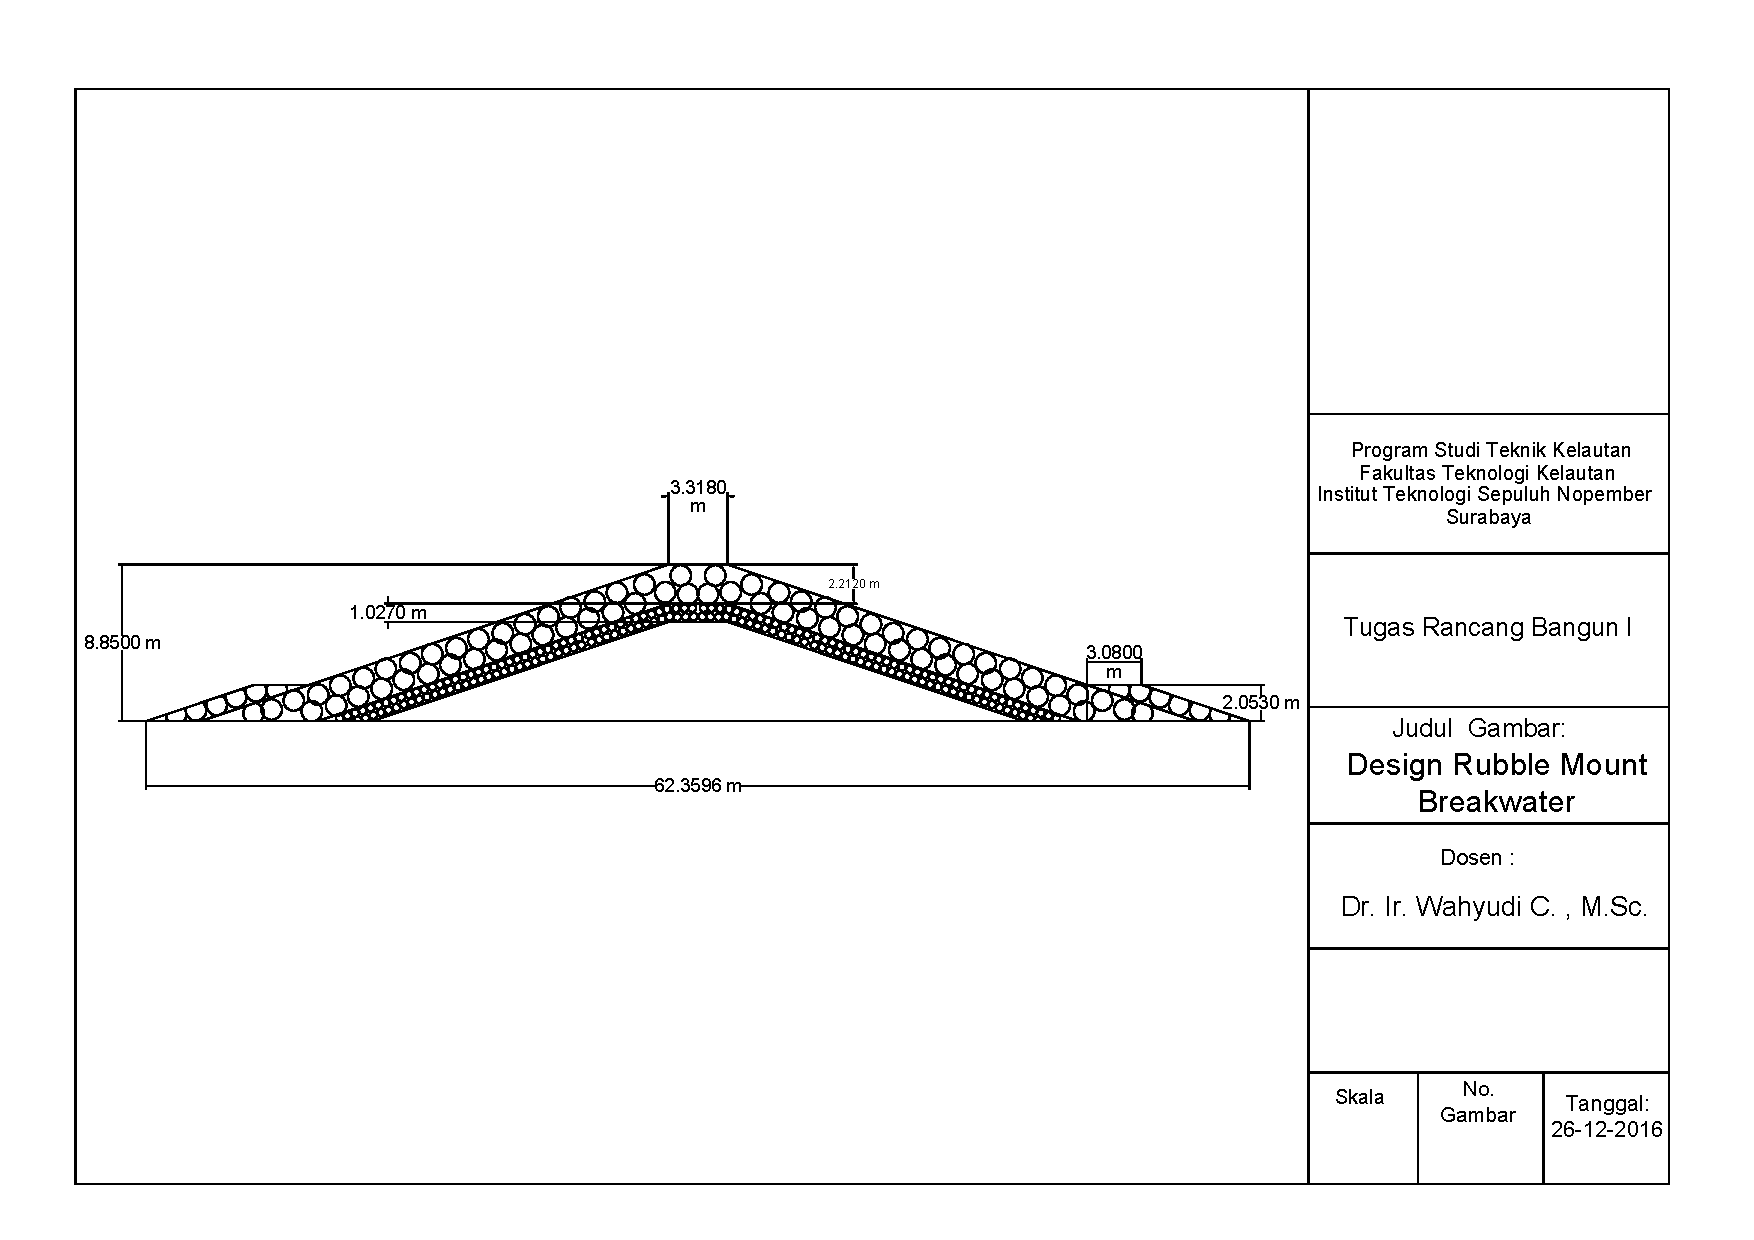
\includepdf{Breakwater.pdf}


\chapter{Kata Pengantar}

\chapter{Abstrak}

\chapter{Abstract}

\tableofcontents

\listoffigures

\listoftables

\lstlistoflistings

\listofappendices





%=================== Main part of document =================%
% Chapters etc
% TODO: Check if spacing is correct
\mainmatter

\begin{doublespace}

% \spacing{1.213}
% Pendahuluan
\subimport{Skripsi/Pendahuluan}{pendahuluan}

% Landasan Teori
\subimport{Skripsi/Landasan_Teori}{landasan_teori}

\chapter{Trial}
\section{Test}
\subsection{A subsection}
\lipsum[1-2]

\begin{pycode}
print("hello world")
\end{pycode}
% manual code listing

\begin{lstlisting}[caption=Manual input, label={listing-java-manual},language=java,style=skripsilisting]
public class HelloWorld {
	public static void main(String[] args) {
		System.out.println("Hello world");
	}
}
\end{lstlisting}

\lstinputlisting[caption=Test java, label={lst:listing-java}, language=java, style=skripsilisting]{Mahasiswa.java}

\chapter{Landasan Teori}
\lipsum[1-2]

\section{Graphs}
\begin{tikzpicture}
	\begin{axis}[
		axis lines = center,
		xlabel = \(x\),
		ylabel = {\(f(x)\)},
		]
		%Below the red parabola is defined
		\addplot [
		domain=-10:10,
		samples=100,
		color=red,
		]
		{x + 1};
		\addlegendentry{\(x + 1\)}
		%Here the blue parabola is defined
		\addplot [
		domain=-10:10,
		samples=100,
		color=blue,
		]
		{-x};
		\addlegendentry{\(-x\)}

	\end{axis}
\end{tikzpicture}

\section{Block quotes}
This part is an example of making a quote. We'll fill it out with stuff so it becomes more than one line without using lorem ipsum
\begin{quote}
	\lipsum[1-2] \parencite{wombat2016} % Parenthesis citation.
\end{quote}

According to \footcite[Quote from][According to me, this is really neat]{lion2010}, this is something. What can we learn from this exercise? Well, if we add another paragraph, bla bla bla bla bla.

Another example of citation is using this \parencite[see][page 12]{wikibook}



\chapter{Another file in another folder}
Well well well, what do we have here?. Use this command in the document body to insert the contents of another file named filename.tex; again this file should not contain any LATEX preamble. LATEX will start a new page before processing the material input from filename.tex. Make sure not to include the extension .tex in the filename, as this will stop the file from being input (the extension can optionally be included with input and import). It is not possible to nest include commands. Each file that gets has its own .aux file storing information of created labels and contents for the table of contents, list of figures, etc. You can use  with a comma separated list of file names (make sure that there are no leading or trailing spaces). If you do this LATEX will only process the files contained in that list. This can be used to enhance compilation speed if you're only working on a small part of a bigger document. Page numbers and cross references will however still work, as the .aux files of left out files will still be processed.
\section{Title}
\lipsum[1-2]


\subimport{New_Chapter}{another_one} % Imports from subdirectory


\end{doublespace}
%================= Back matters ===================%
% Bibliography and attachments



\backmatter

\printbibliography[heading=bibintoc]


\begin{appendices}
	\chapter{something}

	\section{Appendix Code}
	\begin{lstlisting}[language=java, style=skripsilisting]

		public static void main(String[] args) {
			System.out.println("Wooo, cool!");
		}
	\end{lstlisting}

\end{appendices}


\end{document}



